%% Monografia de PCC - Desempenho das Wireless LAN
%%
\documentclass{abnt}

% Incluir Pacotes ------------------------------------------------
\usepackage[utf8]{inputenc}
\usepackage[brazil]{babel}
\usepackage{url}
%\usepackage [latin1] {inputenc}
\usepackage{ae}                         %% Font Encoding T1 (PDF)
\usepackage[dvips]{graphicx}            %% Inclusao de graficos (DVI/PS)
\usepackage[dvips]{geometry}            %% Dimensoes do documento (DVI/PS)
\usepackage{lscape}                     %% Utilizar pagina em landscape
\usepackage{url}                        %% Trata URLs, e-mails e paths
\usepackage[alf]{abntcite}
\usepackage{cite}


%\usepackage[dvipdfm]{hyperref}% permite configurar hiperef
%\hypersetup{colorlinks=true,linkcolor=blue,citecolor=blue}

\renewcommand{\ABNTchapterfont}{\fontfamily{cmr}\fontseries{b}\selectfont}
\renewcommand{\ABNTsectionfont}{\fontfamily{cmr}\fontseries{b}}
\renewcommand{\tituloformat}{\large\bfseries}

\begin{document}
% ----------------------------------------------------------------
% Paginas iniciais
% ----------------------------------------------------------------
% ----------------------------------------------------------------
% Pginas Iniciais ***********************************************
% ----------------------------------------------------------------

% Capa -----------------------------------------------------------

\autor{
Alfredo José de Paula Barbosa - 16890 \\
Michell Stuttgart Faria - 16930 \\
Paulo Vicente Gomes dos Santos - 15993 \\
Orientador: Prof. Dr. Enzo Seraphim
}

\titulo{SAGA Game Library \\
Biblioteca para desenvolvimento \\
de jogos eletrônicos 2D \\
}

\comentario{Monografia apresentada para o Trabalho de Diploma do curso de
Engenharia da Computação da Universidade Federal de Itajubá.}

\instituicao{Universidade Federal de Itajubá - UNIFEI 
\par Instituto de Engenharia de Sistemas e Tecnologias da Informação Engenharia da
Computação}

\local{Itajubá - MG}

\data{}

\capa

\folhaderosto
                    %% Capa e Folha de rosto
\tableofcontents                  %% Sumario
%\listoffigures                    %% Lista de figuras
%\listoftables                     %% Lista de tabelas
%\include{ListaAbrev}             %% Lista de abreviaturas
%\pretextualchapter{Agradecimentos}

\begin{espacosimples}
\noindent A cada mestre das nossas escolas e famílias, que nos guiaram na construção do conhecimento, dos átomos e das células, dos números e das palavras, dos fenômenos da natureza e dos mistérios da alma, da convivência, da responsabilidade e da dedicação. A cada amigo e familiar que estava lá, tanto nas lutas quanto nas vitórias, como esta, pela graça de Deus, de quem é toda a glória. 
\end{espacosimples}                 %% Agradecimentos
%\begin{resumo}

Uma biblioteca de jogos ou \textit{game engine} pode ser vista como um conjunto de recursos e ferramentas para a construção de um jogo. Você pode criar um jogo sem uma biblioteca básica, assim como você pode criar uma mesa de madeira sem pregos, martelos, parafusos, chaves de fenda e serras, mas as vantagens que as ferramentas proporcionam justificam chamá-las de necessárias.
O nível dessas ferramentas varia: algumas \textit{engines} se limitam a códigos, ou seja, constantes, variáveis, funções e classes relacionadas, mas outras contam com interfaces gráficas que possibilitam o desenvolvimento de um jogo sem codificação alguma. De qualquer forma, uma \textit{game engine} precisa proporcionar, no mínimo, ferramentas para manipular sons, imagens (texto, imagens, etc), memória (dados) e controle (teclado, mouse, etc).

\vspace{1em}
\textbf{Palavras-chave}: \textit{game engine}, jogos eletrônicos, ferramentas de desenvolvimento.
\end{resumo}                 %% Resumo
%-----------------------------------------------------------------
% Corpo da Monografia
% ----------------------------------------------------------------
%% ----------------------------------------------------------------
% Introduo e Conceitos Básicos *******************
% ----------------------------------------------------------------
\chapter{Introdução}
\label{cap:indtroducao}
%
Desde os primórdios da humanidade a competição é uma forma de diversão muito popular. O objetivo de qualquer competição é testar uma habilidade individual ou grupal e destacar quem ganha. Embora essa característica ainda seja a mesma, a competição está condicionada a uma evolução que pode ser notada, por exemplo, na corrida: no começo ela era individual e só testava a velocidade e a resistência da pessoa; hoje uma corrida automobilística testa a resistência, a destreza, a inteligência e a tecnologia da equipe.
Mas essa evolução não se da só na complexidade da competição, ela se manifesta da mesma forma na sua abstração. Os jogos de estratégia que nós conhecemos hoje, por exemplo, são versões abstratas das competições físicas. A aptidão física de cada criatura imaginária é determinada por alguma característica interna do jogo, porque o que o jogo de estratégia testa é o raciocínio e a estratégia da pessoa e não a sua capacidade física propriamente dita. O xadrez internacional, simulando uma guerra da Idade Média, é um caso concreto dessa evolução.
Com o avanço da microeletrônica e da computação, no entanto, o jogo de estratégia ganha uma plataforma que pode simular não só um sistema de lógica, mas toda uma realidade virtual. Qualquer jogo pode ganhar uma versão eletrônica. O jogo eletrônico, portanto, não é só uma brincadeira de criança, ele é na verdade o último estágio de um passatempo milenar. Isso se confirma pela movimentação de recursos e ganhos da indústria dos jogos eletrônicos desta geração.
%
%
% ----------------------------------------------------------------
% Motivacao *******************
% ----------------------------------------------------------------
\section{Motivação}
\label{section:motivacao}
%
%
%
Nos últimos anos, o mercado de games do Brasil tem presenciado um crescimento significativo. \cite{e}
O advento dos dispositivos móveis, como \textit{smartphones} e \textit{tablets}, e a possibilidade de comercializar seu produto \textit{online} em lojas virtuais e assim reduzir custos favoreceu, em parte, a redução da pirataria e fez com que o usuário preferisse a compra do produto original a investir em um produto não-original. Essa mudança de comportamento por parte do consumidor fez com que um mercado, que antes era visto como inseguro, passasse a ser considerado um mercado promissor pelas empresas desenvolvedoras de software, incluindo as desenvolvedoras de \textit{games}.
\par
Com o crescimento da área de desenvolvimento de jogos eletrônicos, surge também a necessidade de encontrar mão-de-obra capacitada, necessidade esta que é uma das maiores reclamações das indústrias de desenvolvimento de \textit{games} do Brasil. Por se tratar de uma área de desenvolvimento recente, é difícil encontrar profissionais capacitados na área. Uma das soluções mais simples para esta carência de mão-de-obra é incentivar estudantes, sejam eles de nível técnico ou universitário, a aprender sobre as ferramentas e técnicas mais utilizadas no desenvolvimento de um jogo eletrônico. Assim, torna-se de suma importância a implementação de ferramentas que facilitem o primeiro contato do estudante com essa complexa área de desenvolvimento, motivo este que nos motivou a criaçãoo da \textit{SAGA Game Library}.
%
%
% ----------------------------------------------------------------
% Objetivos *******************
% ----------------------------------------------------------------
\section{Objetivos}
\label{section:objetivos}
%
A \textit{SAGA Game Library} foi desenvolvida tendo em foco o meio acadêmico. Com o aumento do mercado de desenvolvimento de 
jogos eletrônicos no país, surge a necessidade de investir na capacitação de profissionais para atender a essa demanda. Não apenas profissionais do setor precisam estar em constante atualização, mas os agora estudantes e futuros profissionais também precisam de capacitação. É para esse último que é direcionada esta biblioteca de desenvolvimento. Seu objetivo primário é possibilitar ao usuário, seja ele um estudante ou entusiasta, o primeiro contato com o mundo do desenvolvimento de jogos.
%
\par
%
É certo que já existem muitas \textit{game engines}, inclusive em C++, mas o estudo é o piso de todas as descobertas científicas, o que justifica e motiva o desenvolvimento de uma biblioteca de jogos didática. Esta é a nossa proposta: uma camada de orientação a objetos envolvendo a Allegro de uma forma simples e didática. Simplicidade, eficiência e aprendizado são as palavras-chave da \textit{SAGA Game Library}.
%
%
%                   %% INTRODUCAO
% ----------------------------------------------------------------
% Revis�o bibliogr�fica *******************
% ----------------------------------------------------------------
\chapter{Metodologia}
\label{cap:revisao}
%
Uma vez que a proposta inicial do projeto foi decidida, a pr�xima etapa do trabalho consistiu na defini��o de como a biblioteca seria desenvolvida. Com isso em mente, come�amos pelos pontos mais b�sicos: a linguagem de programa��o e a API a ser utilizada para acesso ao hardware.
%
\section{Linguagem de Programa��o}
\label{linguagem}
%
At� a d�cada de 90 cada jogo tinha a sua \textit{engine}, feita para possibilitar a maior efici�ncia no uso da mem�ria e da unidade de 
processamento poss�vel, de acordo com as exig�ncias de cada jogo. Um jogo que s� usava formas geom�tricas, por exemplo, n�o precisava 
tratar imagens na sua \textit{engine}. O n�vel da microeletr�nica e da computa��o j� possibilita o uso de \textit{engines} gen�ricas, 
mas o desenvolvimento de uma ainda demanda uma programa��o muito pr�xima da m�quina. 
\par
� por isso que a escolha da linguagem de programa��o precisa ser feita com cuidado. Considerando o conhecimento da equipe e o prop�sito do 
projeto, que era uma \textit{engine} did�tica, para influenciar o designe e o desenvolvimento de jogos de acordo com o nosso alcance, as linguagens de programa��o selecionadas para a an�lise foram Actionscript, C++, C\# e Java, de acordo com a simplicidade, o poder e a compatibilidade de cada uma.
%
\subsection{Estudo Comparativo}
%
O Actionscript � uma linguagem orientada a objetos desenvolvida pela Macromedia. O que no in�cio era uma ferramenta para controlar anima��es 
se tornou uma linguagem de script t�o complexa que podia ser usada no desenvolvimento de um jogo. Embora essa linguagem ainda seja muito usada 
no desenvolvimento de jogos de web, o que provocou a decis�o contr�ria a ela foi a expectativa de que o HTML 5 viesse a incorporar o Javascript e, 
dessa forma, modificar ou inutilizar o Actionscript.
\par
O C\# (C Sharp) � uma linguagem multi-paradigma da Microsoft feita para o desenvolvimento de sistemas pr�prios para a plataforma .NET. C\# e Java 
compartilham a mesma simplicidade na leitura e na codifica��o, assim como a mesma forma de interpreta��o e compila��o, mas um programa em C\# est� 
mais pr�ximo da m�quina do que um programa em Java. A escolha parecia feita quando n�s entendemos que a liga��o do C\# com a Microsoft poderia 
custar a compatibilidade do nosso jogo.
\par
Java � uma linguagem orientada a objetos desenvolvida pela Sun, hoje possu�da pela Oracle. A sua fama de espa�osa e pesada n�o � coerente com a 
realidade: hoje a linguagem conta com a Compila��o na Hora ou Just in Time Compilation (JIT Compilation ou s� JIT), 
para que a sua execu��o n�o seja mais interpretada. Mas a sua principal caracter�stica � a compatibilidade: a M�quina Virtual do Java ou Java Virtual Machine (JVM) � uma plataforma virtual que pode ser feita compat�vel para qualquer plataforma f�sica.
\par
Por mais evolu�da que seja a JVM, no entanto, o Java n�o admite o acesso � m�quina necess�rio para o desenvolvimento de uma Game Engine, 
sen�o com o uso do C++, por meio da Interface Nativa do Java ou Java Native Interface (JNI). Em outras palavras, para usar o Java, nesse caso, 
n�s ter�amos que usar o C++. Esta, por sua vez, n�o � a mais simples na codifica��o, mas n�o tem limita��o alguma tanto em termos de 
compatibilidade quanto em termos de acesso � m�quina.
%
\subsection{A Escolha: C++}
%
C++ (C Mais Mais ou C Plus Plus) \cite{Novatec} � uma linguagem de programa��o multi-paradigma, com suporte para a programa��o imperativa e a programa��o 
orientada a objetos, de uso geral, desenvolvida por Bjarne Stroustrup, para formar uma camada de orienta��o a objetos sobre a linguagem de 
programa��o C. O C++ possibilita a programa��o de baixo n�vel assim como a programa��o de alto n�vel e por isso � considerado uma linguagem 
de programa��o de n�vel m�dio em termos de proximidade da m�quina.
\par
Na vers�o de 2011, com uma �bvia e construtiva influ�ncia da Biblioteca Boost, o C++ ganha uma s�rie de caracter�sticas, entre as quais podemos
citar: verifica��o de tipo din�mica, estruturas de convers�o e controle de alto n�vel, reflex�o padronizada, uma biblioteca de computa��o paralela 
padronizada, coleta de lixo autom�tica, etc. Com essas mudan�as o C++ ganha em simplicidade, sem, contudo, perder a proximidade da m�quina de outrora. 
%
%
\section{Allegro}
\label{allegro}
%
Nas nossas pesquisas para escolher uma biblioteca com a qual trabalhar, duas se destacaram: a Allegro e a SDL. A SDL (Simple Direct Media Layer - 
Camada de M�dia Direta Simples) � uma biblioteca multim�dia simples de usar, multiplataforma, de c�digo aberto, e amplamente usada para fazer  jogos. 
Ela poderia tamb�m atender as nossas necessidades, mas a Allegro se destacou por ter um c�digo mais limpo e intuitivo, e rotinas espec�ficas 
para o desenvolvimento de jogos, como renderiza��o acelerada por hardware e suporte nativos a diversos formatos de imagens e arquivos de �udio.
Por esta raz�o ela foi escolhida.
\par 
Allegro\cite{AllegroDoc} � uma biblioteca gr�fica multiplataforma, de c�digo fonte aberto e feita na sua maioria em C, mas utilizando internamente tamb�m Assembly e C++. 
Seu nome � um acr�nimo recursivo que representa ``\textit{Allegro Low Level Game Routines}'' (``Rotinas de jogo de baixo n�vel Allegro'').
Funciona em diversos compiladores e possui rotinas para a manipula��o de fun��es multim�dia de um computador, al�m de oferecer um ambiente ideal 
para o desenvolvimento de jogos, tornando-se uma das mais populares ferramentas para esse fim atualmente. Originalmente desenvolvida por 
Shawn Hargreaves, ela se tornou um projeto colaborativo, com colaboradores de todo o mundo.
\par
Ela possui fun��es para jogos 2D e 3D, mas n�o � indicada para o �ltimo caso. Apesar de n�o ser suficiente para o completo desenvolvimento 
de um jogo, existem pequenas bibliotecas adicionais (add-ons), feitas para serem acopladas � Allegro, permitindo assim a sua extens�o. Atrav�s 
desses add-ons � poss�vel, por exemplo, obter suporte a arquivos MP3, GIF, imagens JPG e v�deos AVI.
\par
Internamente, a biblioteca � divida em blocos. Isso � �til para que o usu�rio n�o tenha que colocar uma por��o de fun��es que n�o usa na hora 
de distribuir seu jogo, incluindo somente as partes que for utilizar, diminuindo consideravelmente o tamanho do mesmo.
\par
Atualmente a biblioteca se encontra na sua quinta vers�o. Allegro 5 foi completamente reescrita de suas vers�es anteriores. Foi feito um esfor�o 
para tornar a API mais consistente e segura, o que trouxe melhorias funcionais e uma grande mudan�a na sua arquitetura, sendo agora orientada 
a eventos. Entretanto n�o � compat�vel com suas vers�es antigas.
\par
A Allegro 5.0 suporta as seguintes plataformas:
\begin{itemize}
 \item Windows (MSVC, MinGW);
 \item Unix/Linux;
 \item MacOS X;
 \item iPhone;
 \item Android (Suporte provido pela Allegro 5.1, que ainda se encontra inst�vel).
\end{itemize}
%
%
\subsection{Principais Recursos e Fun��es}
%
A seguir, encontramos um conjunto dos principais recursos da Allegro 5, come�ando com
as fun��es mais gerais da biblioteca.
%
\begin{itemize}
 \item \textbf{al\_init()}: Inicializa a biblioteca Allegro, dando valores a algumas vari�veis globais e reservando mem�ria. 
 Deve ser a primeira fun��o a ser chamada.
 \item \textbf{al\_exit()}: Encerra a Allegro. Isto inclui retornar ao modo texto e remover qualquer rotina que tenha sido instalada. 
 N�o h� necessidade de chamar essa fun��o explicitamente, pois, normalmente, isto � feito quando o programa termina.
\end{itemize}
%
As rotinas de video:
%
\begin{itemize}
 \item \textbf{ALLEGRO\_DISPLAY}: Tipo que representa a janela principal. A biblioteca permite que se trabalhe com m�ltiplas janelas.
 \item \textbf{al\_create\_display(width, height)}: Cria uma inst�ncia da janela, retornando um ponteiro para ALLEGRO\_DISPLAY. 
 Os par�metros indicam as dimens�es em pixels.
 \item \textbf{al\_flip\_display()}: Fun��o para atualizar a tela.
 \item \textbf{al\_destroy\_display(var)}: Finaliza a inst�ncia \textit{var} do tipo ALLEGRO\_DISPLAY\*.
\end{itemize}
%
As rotinas para manipula��o de arquivos de imagem:
%
\begin{itemize}
 \item \textbf{ALLEGRO\_BITMAP}: Tipo que representa o arquivo de imagem carregado pela Allegro.
 \item \textbf{al\_init\_image\_addon()}: Inicializa o add-on da Allegro 5 para utiliza��o de imagens.
 \item \textbf{al\_load\_bitmap(``example.jpg'')}: Carrega a imagem indicando no par�metro o nome e tipo. Ela deve estar previamente salva na pasta 
 do programa. Recebe o caminho relativo ou absoluto da imagem a ser carregada, retornando um ponteiro para o tipo ALLEGRO\_BITMAP.
 \item \textbf{al\_draw\_bitmap(bitmap, x, y, mirror)}: Fun��o para desenhar a imagem na tela. Os par�metros s�o o bitmap a ser desenhado, as 
 posi��es x e y e as flags de espelhamento (0, ALLEGRO\_FLIP\_HORIZONTAL, ALLEGRO\_FLIP\_VERTICAL).
\end{itemize}
% 
As rotinas de �udio:
%
\begin{itemize}
 \item \textbf{ALLEGRO\_SAMPLE}: Tipo que representa arquivos pequenos, geralmente efeitos sonoros.
 \item \textbf{ALLEGRO\_AUDIO\_STREAM}: Tipo para representar arquivos grandes, de forma que o arquivo n�o � carregado de uma vez para a 
 mem�ria. Geralmente representa os arquivos que ir�o compor uma trilha sonora.
 \item \textbf{al\_install\_audio()} e \textbf{al\_init\_acodec\_addon()}: A primeira inicializa as fun��es relativas ao �udio. A segunda inicializa os 
 codecs necess�rios para carregar os diversos formatos de arquivo suportados. Fornece suporte a alguns formatos, como Ogg, Flac e Wave.
 \item \textbf{al\_set\_audio\_stream\_playing(musica, true)}: Fun��o que recebe o arquivo de �udio j� carregado no primeiro par�metro e um tipo 
 booleano no segundo (true para faz�-la tocar ou false, em caso contr�rio).
 \item \textbf{al\_destroy\_audio\_stream(musica) } e \textbf{al\_destroy\_sample(sample)}: Fun��es de desaloca��o dos arquivo de �udio carregados 
 pela Allegro.
\end{itemize}
%
%
A Allegro ainda possui muitos recursos que n�o foram citados por fugirem do escopo deste cap�tulo. Posteriormente,
n�s iremos explorar mais a fundo os recursos que a Allegro oferece.
%
%
\section{O software Tiled}
\label{tiled}
%
A grande maioria dos jogos eletr�nicos 2D apresenta, al�m dos \textit{sprites} dos personagens e itens, uma imagem representando o cen�rio do jogo.
Dependendo da natureza do jogo, esses cen�rios podem possuir grandes dimens�es, o que torna custoso para o software do jogo carregar e 
armazenar essa imagem em mem�ria (RAM e em disco). Mas, se analisarmos a imagem que representa o cen�rio, vamos verificar que o mesmo � formado
por pequenas partes que se repetem com muita frequ�ncia. Assim, aproveitando dessa caracter�stica e com o objetivo de diminuir o consumo de
mem�ria e o desempenho ao carregar imagens de resolu��o elevada, foi desenvolvida uma t�cnica conhecida como \textit{TileMap}. A t�cnica
consiste no uso de uma imagem, chamada \textit{tileset}, contendo pequenos peda�os de imagens, conhecidos como \textit{tiles}, que s�o
as imagens que se repetem em grande quantidade na imagem do cen�rio de jogo. Estes \textit{tiles} s�o usados 
para criar uma imagem composta denominada \textit{tiled layer}.
%
%
\begin{figure}[H]
    \centering
    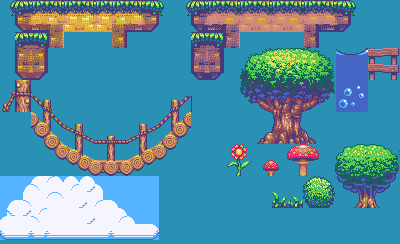
\includegraphics[scale = 1.0]{Imagens/tileset_edit.png}
    \caption{\textit{Exemplo de \textit{tileset}.}}
    \label{tileset_example}
\end{figure}
%
\par
%
O cen�rio final do jogo pode ser constitu�do de um �nico \textit{tiled layer} ou ser resultante da combina��o 
de dois ou mais \textit{tiled layers}. Atrav�s da t�cnica de \textit{Tilemap}, torna-se poss�vel construir in�meros cen�rios,
com variadas dimens�es, usando como base o mesmo \textit{tilesets}, aumentando a economia de mem�ria e n�o reduzindo o desempenho 
no carregamento de imagens.
%
%
%
\begin{figure}[H]
    \centering
    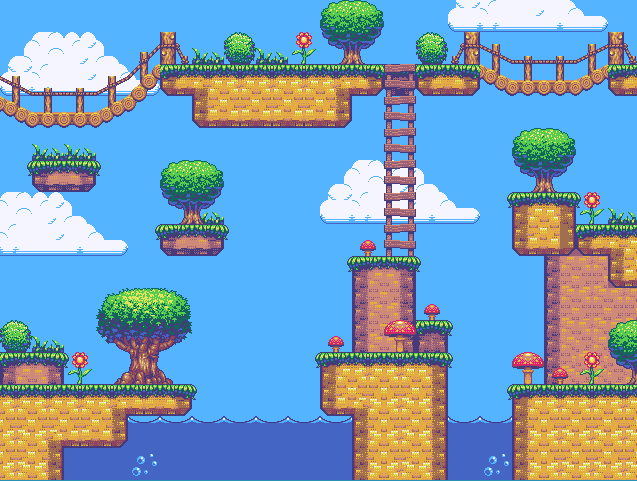
\includegraphics[scale = 0.65]{Imagens/cenario.png}
    \caption{\textit{Exemplo de um cen�rio constru�do com tileset.}}
    \label{cenario_example}
\end{figure}
%
%
\par
O software Tiled \cite{SiteTiled} � uma ferramenta gratuita desenvolvida em C++ para a cria��o de layouts e mapas usando \textit{tilesets}
baseado na t�cnica de \textit{Tilemap}. De simples manuseio e grande versatilidade, o Tiled faz a edi��o de v�rias camadas 
de \textit{tiles} e salva tudo em um formato padronizado de extens�o ``.tmx''. Uma das principais vantagens do formato TMX � sua organiza��o, 
detalhamento e praticidade, sendo que seu conte�do pode ser lido atrav�s do uso de um \textit{parser} para arquivos XML.
%
\begin{figure}[H]
    \centering
    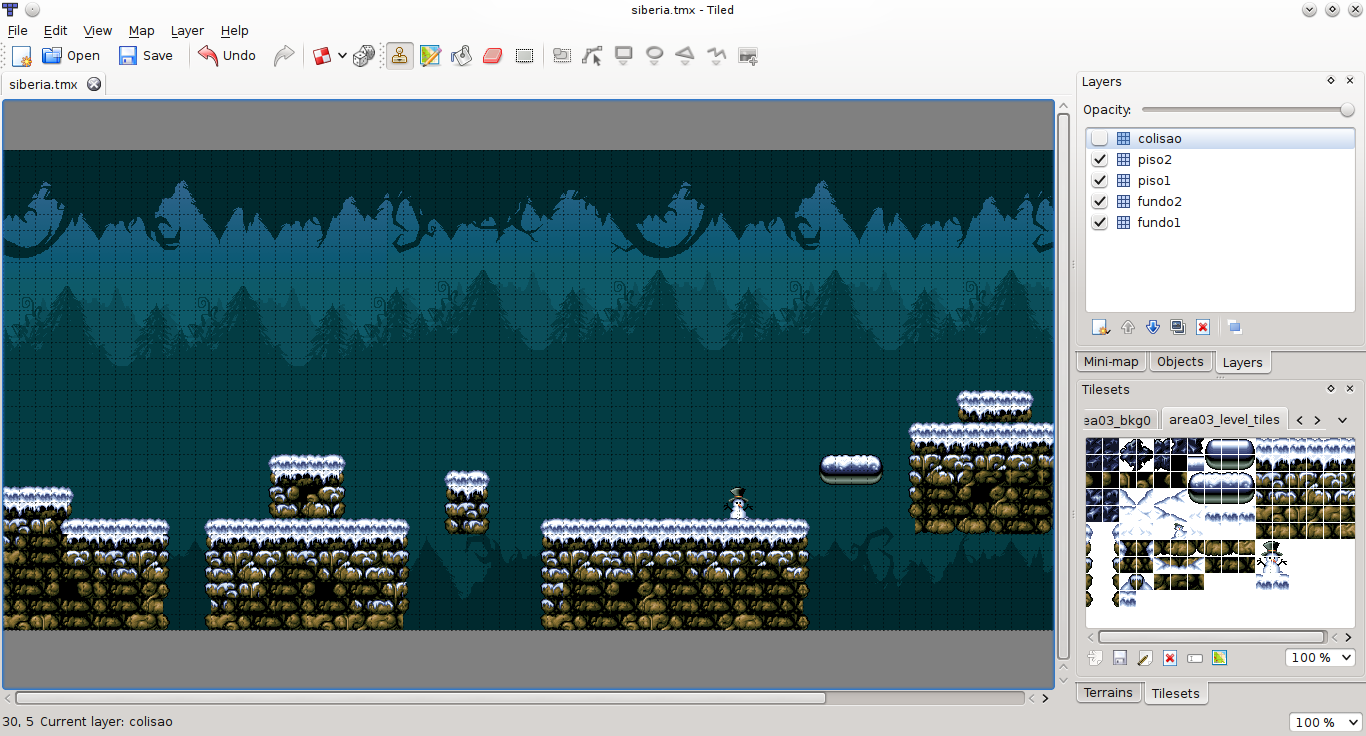
\includegraphics[scale = 0.45]{Imagens/Tiled.png}
    \caption{\textit{Interface do \textit{software} Tiled.}}
    \label{tiled_interface}
\end{figure}
%
\par
O Tiled � um editor de n�veis que suporta mapas com proje��es ortogonais e isom�tricas e ainda permite que 
objetos personalizados sejam salvos como imagens na resolu��o que desejar. Tem suporte tamb�m a comandos externos, 
\textit{plugins} e formatos usados por outros editores. � compat�vel 
com diversas \textit{engines} de cria��o de jogos e fornece meios de comprimir seus dados de modo a diminuir o tamanho em disco do arquivo TMX.
� poss�vel, ainda, redimensionar e alterar o mapa posteriormente, criar m�ltiplos mapas em uma �nica sess�o e ainda salvar ou 
restaurar at� nove vezes. Com ele pode-se especificar o tamanho de cada \textit{tile} em um \textit{tileset}, ou criar um mapa sem tamanho estrito 
sobre as imagens \cite{TiledTutorial}.
Mesmo que o desenvolvedor n�o queira que seu jogo seja baseado em \textit{tiles}, o software � ainda uma excelente escolha como um editor 
de n�veis. Pode-se us�-lo tamb�m nas entidades invis�veis, tais como �reas de colis�o e o aparecimento de objetos dentro do 
mapa. Por sua simplicidade ela pode ser usada por programadores iniciantes ou experientes.
\par 
O processo de cria��o de um mapa com o Tiled � feito basicamente usando os passos abaixo:
%
\begin{enumerate}
 \item Escolher o tamanho do mapa e tamanho do \textit{tile} base;
 \item Adicionar \textit{tilesets} vindos de imagens;
 \item Adicionar quaisquer objetos que representem algo abstrato;
 \item Salvar o mapa no format TMX;
 \item Importar o arquivo TMX e interpret�-lo para o jogo.
\end{enumerate}
%%
O Tiled � totalmente gratuito. Esse detalhe aliado � sua facilidade de uso e versatilidade, tornaram-no extremamente popular em meio
� comunidade de desenvolvedores de jogos, onde n�o s� estudantes e entusiastas, mas tamb�m empresas e profissionais da �rea, passaram a adot�-lo 
como editor de n�veis padr�o. Seguindo esse pensamento, o nosso \textit{framework} a ser desenvolvido tamb�m possui suporte nativo
aos n�veis constru�dos usando esse software.
%
Um dos recursos mais interessantes do Tiled � a possibilita de exportar os dados contidos no arquivo .tmx de forma compactada e codifica��o. 
A principal vantagem do uso dos algoritmos compacta��o e codifica��o � a redu��o do tamanho em disco do
arquivo .tmx resultante e aumento da velocidade de carregamento do cen�rio, uma vez que a biblioteca carrega os dados codificados e/ou compactados
e os decodifica/descompacta a n�vel de software ao inv�s de realizar a leitura dos mesmo em disco. 
\par 
A compacta��o de dados fornecida pelo Tiled � realizada pelas bibliotecas ZLIB e GZIP, enquanto a codifica��o � realizada pelo algoritmo Base64.
S�o fornecidas as op��es de exportar os dados no arquivo .tmx na forma codificada e compactada ou apenas na forma codificada. Tamb�m s�o oferecidas as op��es de exportar os dados em formato puro (sem codifica��o) XML ou no formato CVS. 
\par 
A seguir podemos verificar a redu��o do tamanho em disco de um arquivo .tmx em rela��o ao seu tamanho em disco sem codifica��o/compacta��o.
%
\begin{itemize}
 \item Arquivo XML puro( sem codifica��o/compacta��o): 31,3 KB;
 \item Com codifica��o Base64: 9,6 KB;
 \item Com codifica��o Base64 + GZIP: 2,2 KB;
 \item Com codifica��o Base64 + ZLIB: 2,1 KB;
 \item No formato CVS: 4,9 KB.
\end{itemize}
%
A \textit{SAGA Game Library} prove suporte total e otimizado as 5 op��es de exporta��o acima. Ela, assim com o Tiled, tamb�m faz
uso das bibliotecas GZIP e ZLIB para descompacta��o e tamb�m realiza a decodifica��o dos dados em Base64 contidos no arquivo .tmx. 
%
%
%
\section{A biblioteca TinyXML}
\label{tinyXML}
%
� uma biblioteca escrita em C++ que analisa uma sequ�ncia de entrada no formato XML e cria uma estrutura independente 
de plataforma ou linguagem. Em outras palavras, ela realiza o \textit{parser} de uma arquivo .xml e armazena a informa��o 
em objetos C++ que podem ser manipulados livremente. 
\par 
A TinyXML\cite{TinyXMLTutorial} pode ser facilmente integrada em outros programas, bastando apenas adicionar seus 
arquivos ao projeto. Com ela � poss�vel realizar o acesso aos dados direta ou iterativamente, altera��o da estrutura atrav�s 
de inser��o e remo��o de elementos, remo��o de espa�os duplicados e a grava��o para ficheiros em formato XML.
TinyXML � uma estrutura extremamente compacta e robusta, elaborada para um r�pido e f�cil aprendizado. Pode ser usada para 
fins de c�digo aberto ou comerciais. Ela � compat�vel com UTF-8, de modo a permitir que arquivos XML sejam manipulados em 
qualquer linguagem.
\par
No \textit{framework} que ser� desenvolvido, a TinyXML ser� respons�vel por realizar o \textit{parser} do arquivo .tmx gerado
pelo software Tiled.
%
%

                   %% Como escrever um projeto de pesquisa
% ----------------------------------------------------------------
\bibliographystyle{abnt-alf}
\bibliography{biblio}             %% REFERENCIAS (deve-se possuir o arquivo do tipo bibitex)
% ----------------------------------------------------------------
\end{document}
% ----------------------------------------------------------------
